\documentclass{beamer}
\setbeamertemplate{navigation symbols}{}
\usepackage{comment}

\setbeamercolor{frametitle}{fg=black,bg=white}
\setbeamercolor{title}{fg=black,bg=yellow!85!orange}
\usetheme{AnnArbor}

\usepackage{textpos} % package for the positioning
\usepackage{listings}
\usepackage{xcolor}
\usepackage[most]{tcolorbox}
\usepackage{mathtools}
\usepackage{graphicx}
\usepackage{graphbox}
\usepackage{movie15}
\usepackage{caption}
\DeclareCaptionType{code}[Code Listing][List of Code Listings] 

\definecolor{codegreen}{rgb}{0,0.6,0}
\definecolor{codegray}{rgb}{0.5,0.5,0.5}
\definecolor{codepurple}{rgb}{0.58,0,0.82}
\definecolor{backcolour}{rgb}{0.95,0.95,0.92} 
\lstdefinestyle{mystyle}{
    backgroundcolor=\color{backcolour},   
    commentstyle=\color{codegreen},
    keywordstyle=\color{magenta},
    numberstyle=\tiny\color{codegray},
    stringstyle=\color{codepurple},
    basicstyle=\ttfamily\footnotesize,
    breakatwhitespace=false,         
    breaklines=true,                 
    captionpos=b,                    
    keepspaces=true,                 
    numbers=left,                    
    numbersep=5pt,                  
    showspaces=false,                
    showstringspaces=false,
    showtabs=false,                  
    tabsize=2
}

\lstset{style=mystyle}

\lstdefinelanguage
   [x64]{Assembler}     % add a "x64" dialect of Assembler
   [x86masm]{Assembler} % based on the "x86masm" dialect
   % with these extra keywords:
   {morekeywords={CDQE,CQO,CMPSQ,CMPXCHG16B,JRCXZ,LODSQ,MOVSXD, %
                  POPFQ,PUSHFQ,SCASQ,STOSQ,IRETQ,RDTSCP,SWAPGS, %
                  rax,rdx,rcx,rbx,rsi,rdi,rsp,rbp, %
                  r8,r8d,r8w,r8b,r9,r9d,r9w,r9b, %
                  r10,r10d,r10w,r10b,r11,r11d,r11w,r11b, %
                  r12,r12d,r12w,r12b,r13,r13d,r13w,r13b, %
                  r14,r14d,r14w,r14b,r15,r15d,r15w,r15b}} %


\beamersetuncovermixins{\opaqueness<1>{25}}{\opaqueness<2->{15}}

%Copyright
\addtobeamertemplate{frametitle}{}{%
\begin{textblock*}{50mm}(0cm,-1.25cm)
\color{yellow!85!orange}
\tiny{Copyright \copyright 2024 CNM.}
\end{textblock*}}

% position the logo
\addtobeamertemplate{frametitle}{}{%
\begin{textblock*}{100mm}(11.4cm,-1.3cm)

\includegraphics[height=1cm,width=1cm,keepaspectratio]{fig/ddclogotransparent.png}
\end{textblock*}}

\AtBeginSection[]{
  \begin{frame}
  \vfill
  \centering
  \begin{beamercolorbox}[sep=8pt,center,shadow=true,rounded=true]{title}
    \usebeamerfont{title}\insertsectionhead\par%
  \end{beamercolorbox}
  \vfill
  \end{frame}
}

\begin{document}
\title{Quantum Technician Bootcamp}
\author{Brian Rashap}
\date{September 2025} 

\begin{frame}
\titlepage
\end{frame}

\section{Geometric Optics}

\begin{frame}\frametitle{Ray Nature of Light}
The word "ray" means a straight line that originates at some point.

\begin{center}
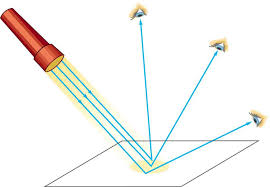
\includegraphics[width=6cm]{fig/rays.jpg}
\end{center}

The part of optics dealing with the ray aspect of light is called "geometric optics."

\end{frame}


\begin{frame}\frametitle{Reflection}
The angle of reflection equals the angle of incidences

\begin{center}
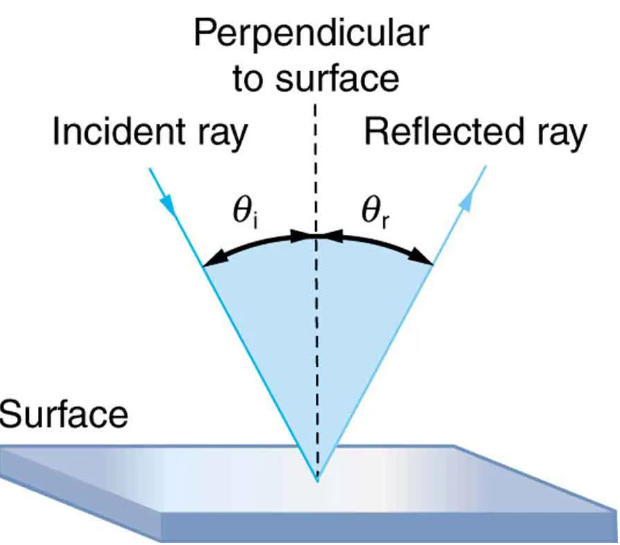
\includegraphics[width=6cm]{fig/reflect.png}
\end{center}

\end{frame}

\begin{frame}\frametitle{Demonstration: Handling Optics}
\begin{center}
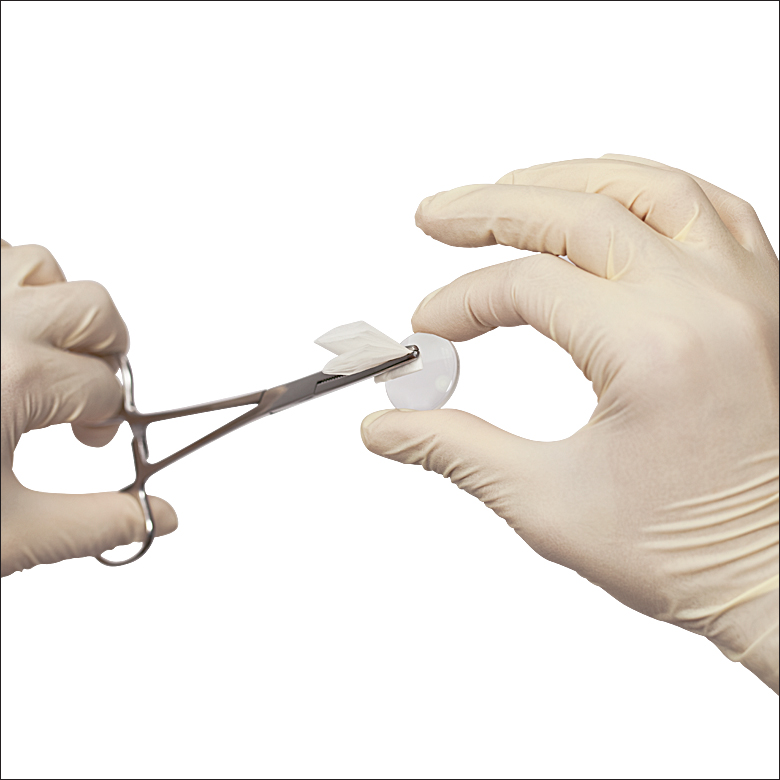
\includegraphics[width=6cm]{fig/opticscleaning.jpg}
\end{center}
\end{frame}

\begin{frame}\frametitle{Assignment: Laser Tag}
\begin{columns}
\begin{column}{5cm}
\begin{center}
\includegraphics[width=4.5cm]{fig/lasertag.jpg}
\end{center}
\end{column}
\begin{column}{7cm}
\begin{itemize}
\item Align a Laser and a target at opposite ends of the table.
\item When obstacles are placed in the path, without adjusting laser, add mirrors to get the beam to the target.
\end{itemize}
\end{column}

\end{columns}
\end{frame}




\begin{frame}\frametitle{Rough vs Smooth Surfaces}

\begin{center}
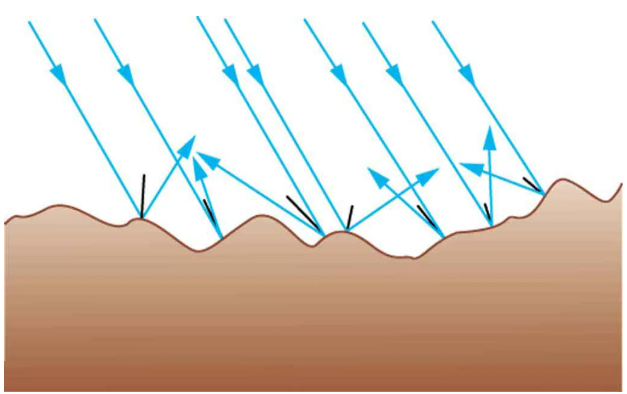
\includegraphics[width=3.5cm]{fig/reflect_rough.png}
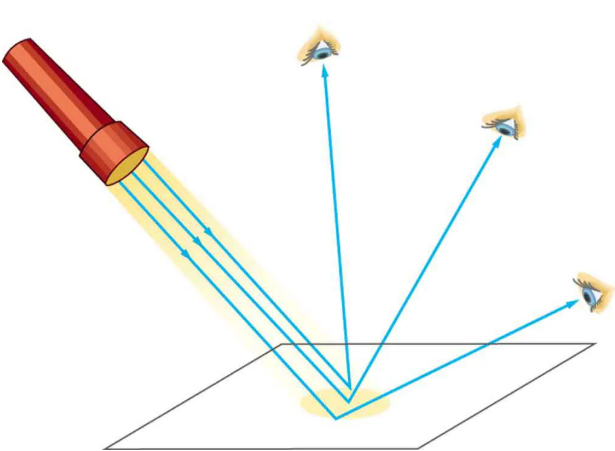
\includegraphics[width=3.5cm]{fig/reflect_paper.png}
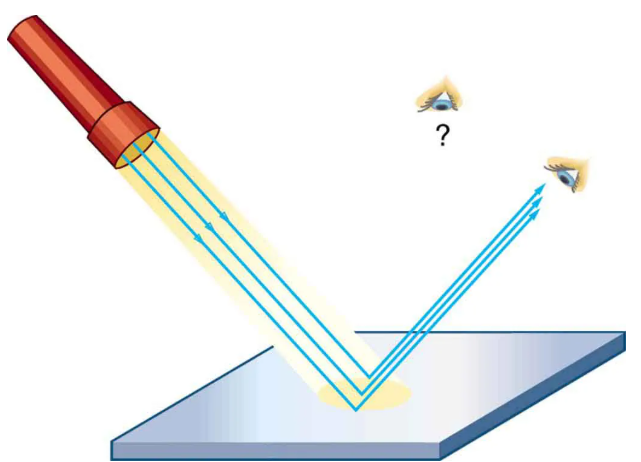
\includegraphics[width=3.5cm]{fig/reflect_mirror.png}
\end{center}

\end{frame}

\begin{frame}\frametitle{Mirrors and Virtual Images}
When we see ourselves in a mirror, it appears that our image is actually behind the mirror.

\begin{center}
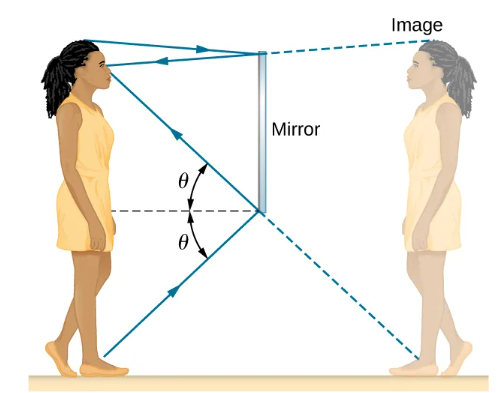
\includegraphics[width=6cm]{fig/virtual.png}
\end{center}

\end{frame}

\begin{frame}\frametitle{Speed of Light}
\begin{columns}
\begin{column}{7cm}
\begin{itemize}
\item In 1676, Danish astronomer Ole Roemer noted the change in orbital period of Jupiter's moons depending of if the earth was moving towards or away from Jupiter. He as able to calculate speed of light to be $2.26 x 10^8 (\frac{m}{s})$.
\item In 1887, American physicist Albert Michelson used a rotating mirror to get a more precise measurement of the speed of light. 
\item Today, the speed of light is known as:
\end{itemize}
\begin{center}
$c=2.99792458×10^8 (\frac{m}{s})$.
\end{center}

\end{column}
\begin{column}{5cm}
\begin{center}
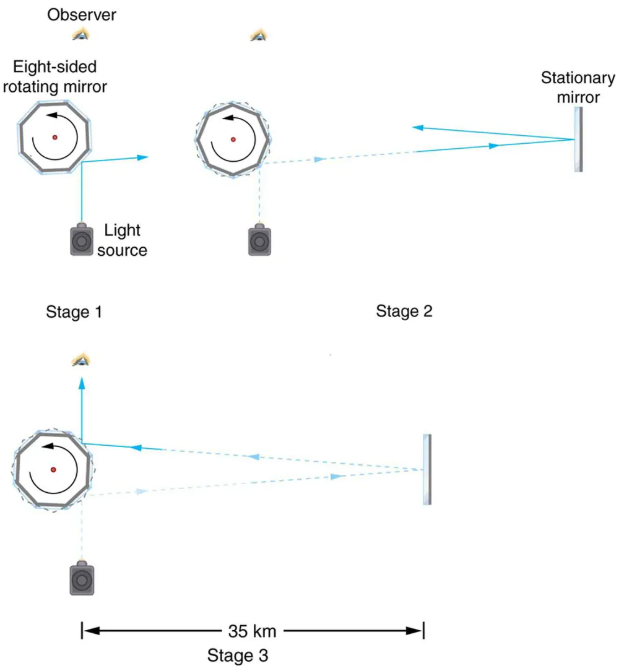
\includegraphics[width=4.5cm]{fig/c_meas.png}
\end{center}
\end{column}
\end{columns}
\end{frame}

\begin{frame}\frametitle{Assignment: Two Mirror Walk}
\begin{columns}
\begin{column}{4cm}
\begin{center}
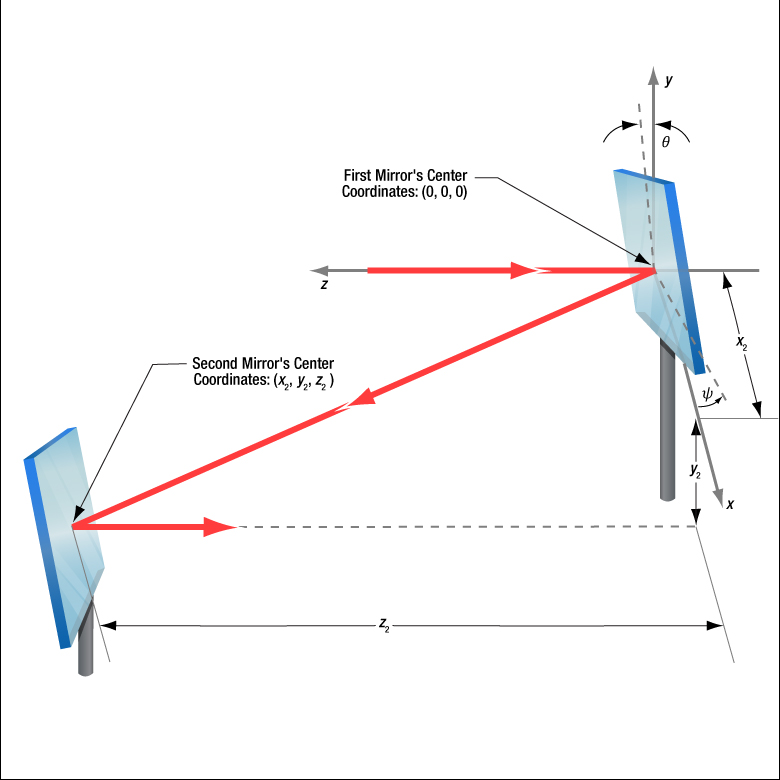
\includegraphics[width=3cm]{fig/twoMirror.jpg}

\vspace{1cm}
\includegraphics[width=4cm]{fig/twoMirror2.jpg}

\end{center}
\end{column}
\begin{column}{7.5cm}
\begin{enumerate}
\item Setup: Laser, $45^{\circ}$ mirror, second $45^{\circ}$ mirror, two irises, target.
\item Adjust first mirror to center beam on center iris 1
\item Open iris 1, adjust second mirror to center beam on iris 2
\item Iterate steps 2 and 3 until the beam passes through the center of both iris and hits target.
\end{enumerate}
\end{column}
\end{columns}

\end{frame}

\section{Math Interlude: Trigonometry}

\begin{frame}\frametitle{Algebraic Functions}
\begin{columns}
\begin{column}{4.5cm}
An algebraic function provides a "y-value" for every "x-value"
\begin{itemize}
\item Linear: $y = x + 2$
\item Quadratic: $y = x^2$
\item Periodic: $y = sin(x)$
\end{itemize}
\end{column}
\begin{column}{7cm}
\begin{center}
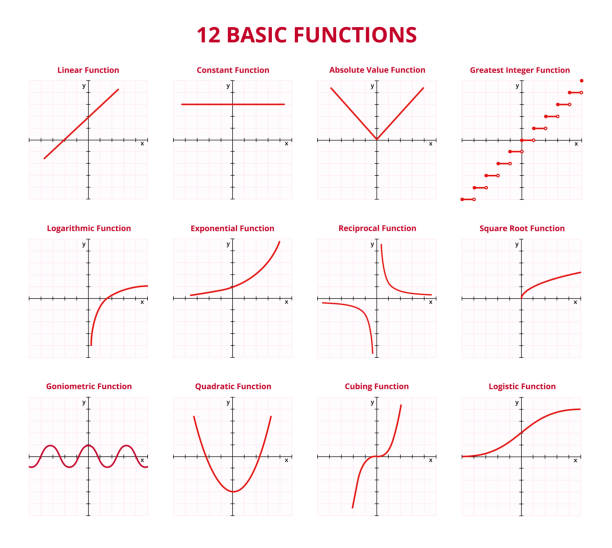
\includegraphics[width=7cm]{fig/basicfun.jpg}
\end{center}
\end{column}
\end{columns}
\end{frame}

\begin{frame}\frametitle{More Desmos Fun}

\begin{center}
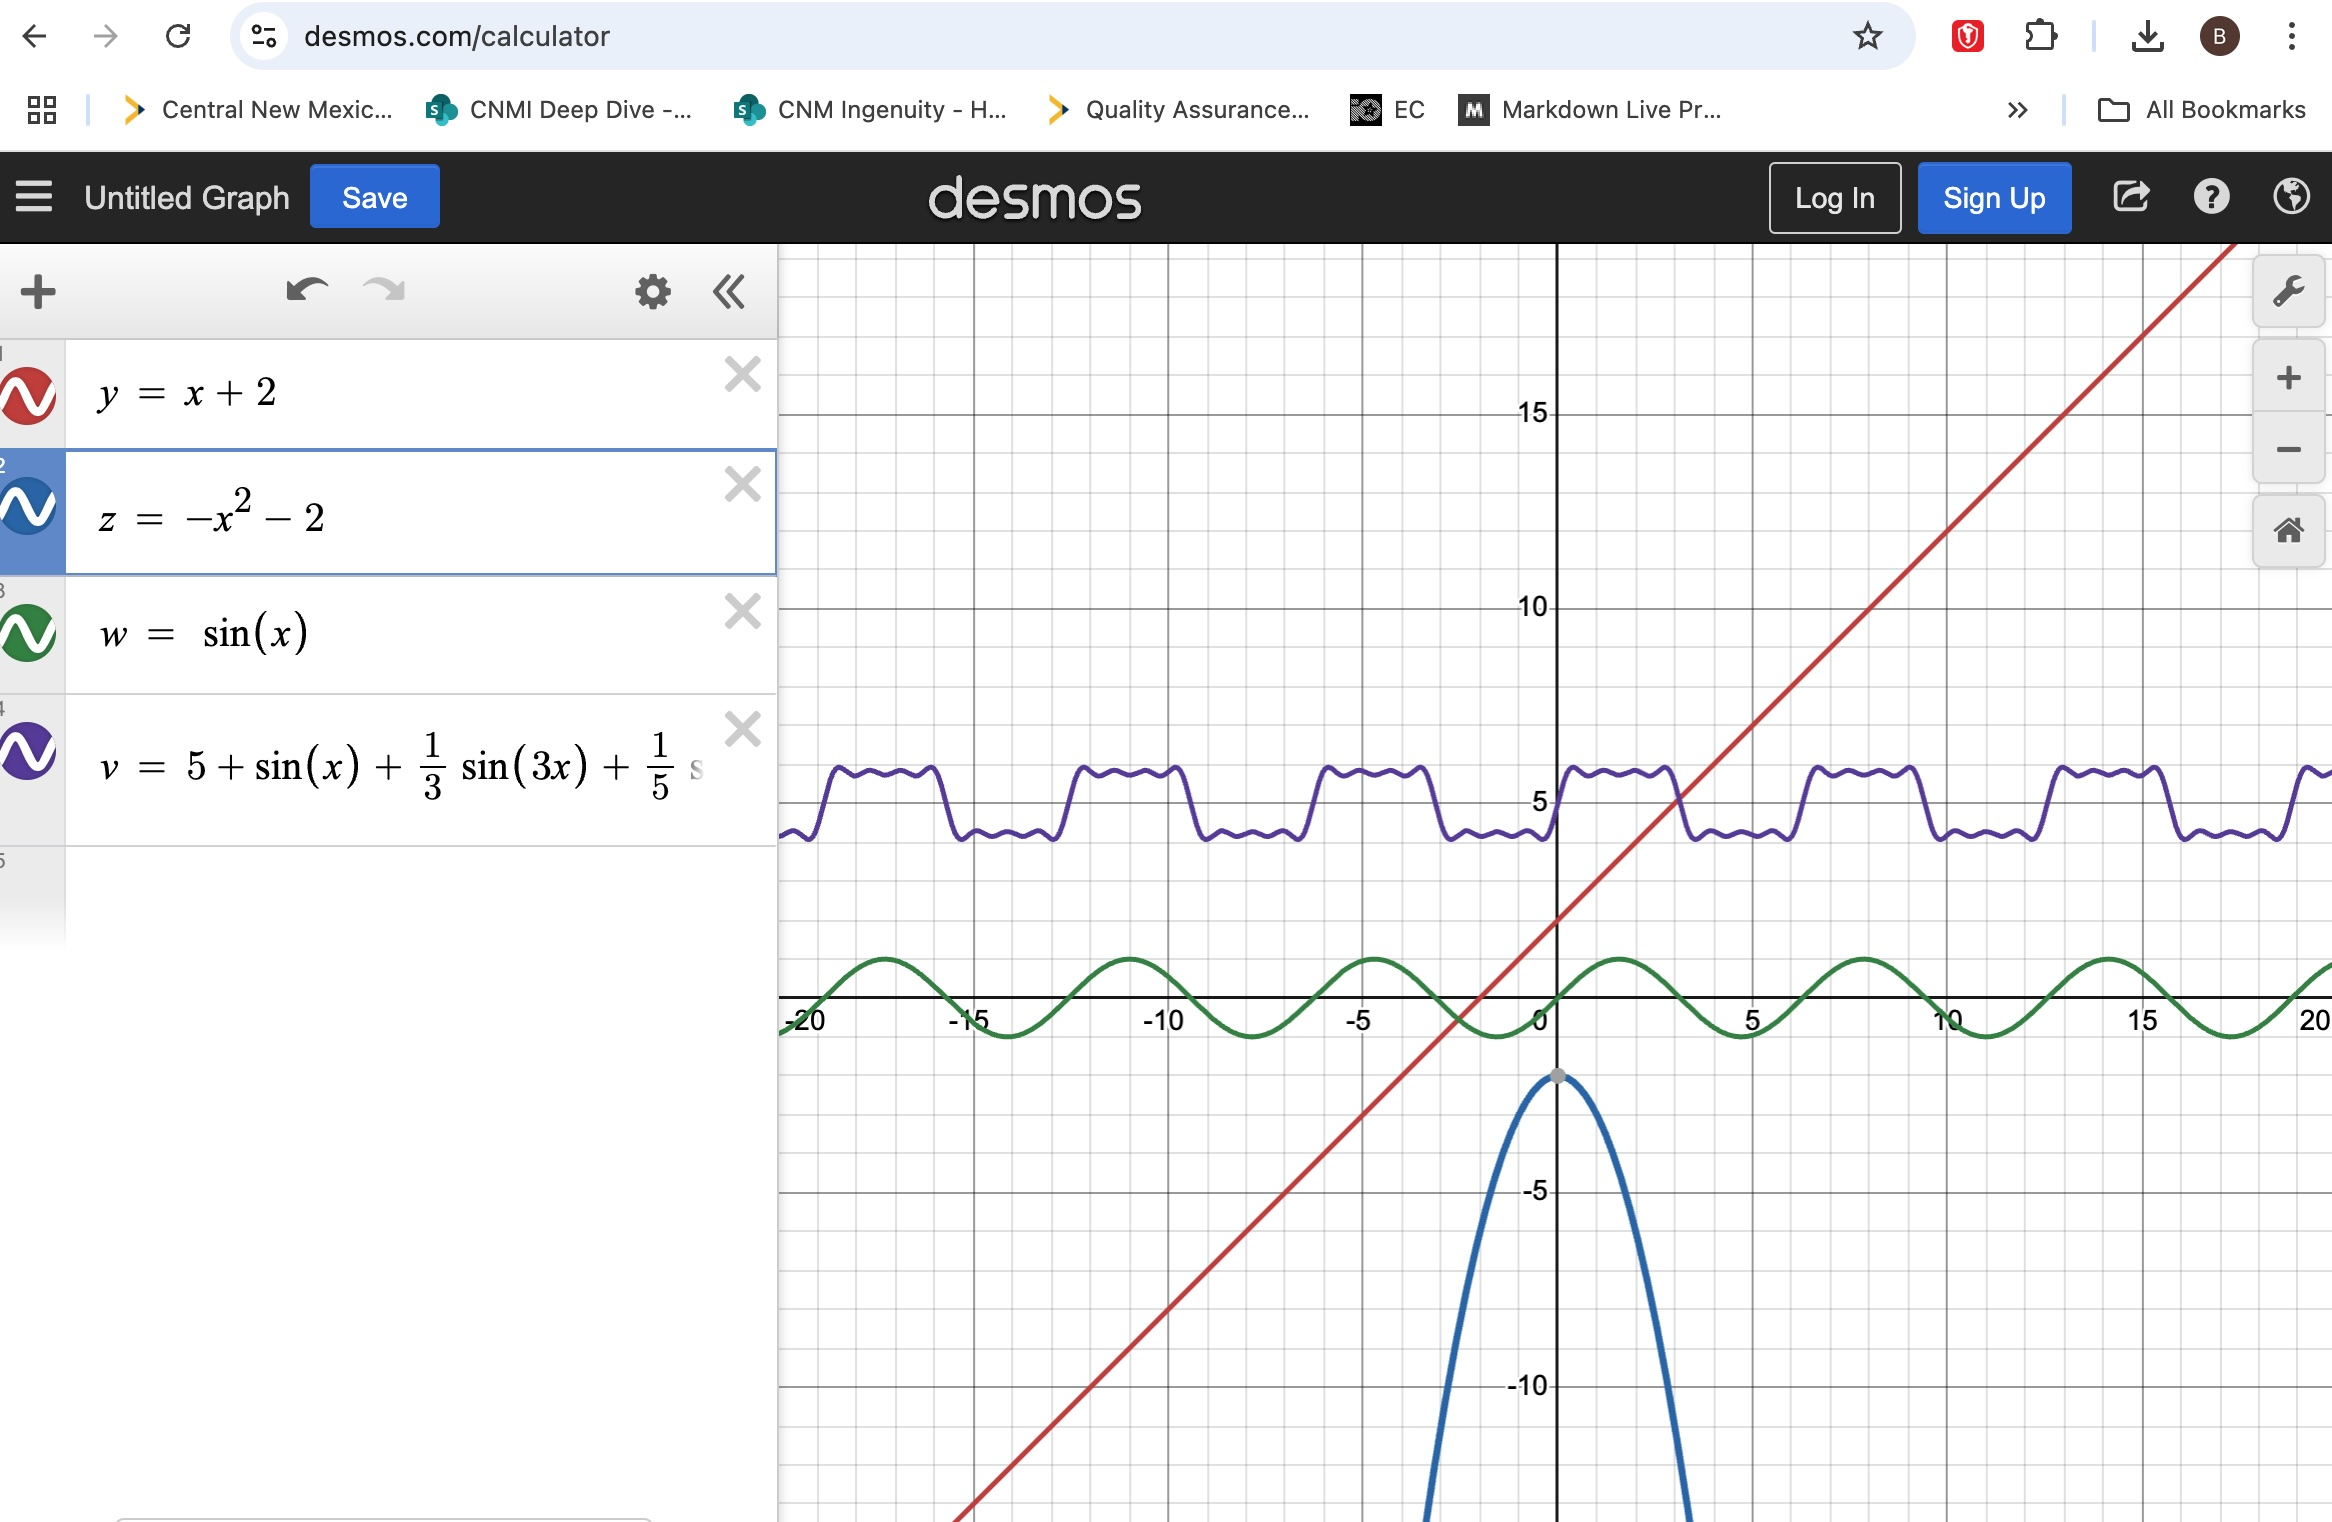
\includegraphics[width=12cm]{fig/desmosfun.jpg}
\end{center}
\end{frame}


\begin{frame}\frametitle{Pi ($\pi)$}

\begin{center}
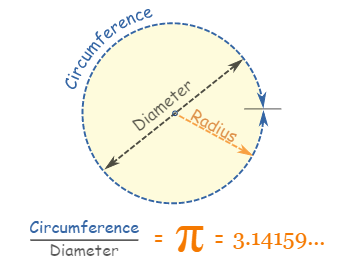
\includegraphics[width=8cm]{fig/pi.png}
\end{center}

\end{frame}


\begin{frame}\frametitle{Unit Circle and Trigonometric Functions}
The Unit Circle is a circle with a radius of 1.
\begin{columns}
\begin{column}{6cm}
\begin{center}
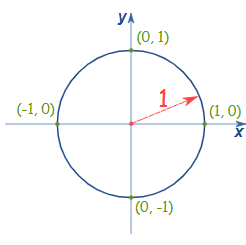
\includegraphics[scale=0.75]{fig/unitcircle.png}
\end{center}
\end{column}
\begin{column}{6cm}
\begin{center}
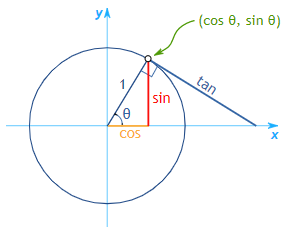
\includegraphics[scale=0.75]{fig/unitcircle_cst.png}
\end{center}
\end{column}
\end{columns}
The Unit Circle can be used to map out the trigonometric values of sine, cosine, and tangent.
\end{frame}


\begin{frame}\frametitle{Unit Circle and the Value of $sin(\theta)$}
\begin{columns}
\begin{column}{6cm}
\begin{center}
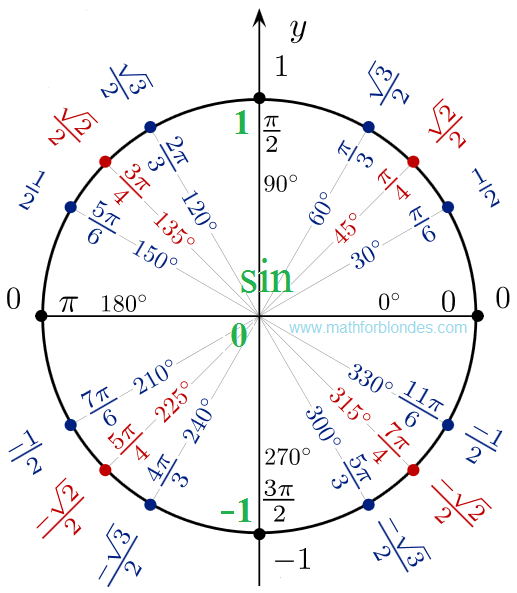
\includegraphics[scale=0.25]{fig/unitcircle_sin.png}
\end{center}
\end{column}
\begin{column}{6cm}
\begin{center}
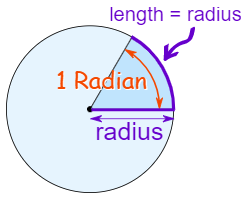
\includegraphics[scale=0.75]{fig/unitcircle_rad.png}
\end{center}
\end{column}
\end{columns}

\vspace{0.25cm}

\begin{itemize}
\item $sin(\theta)$ is the y-value of the point on the Unit Circle at angle $\theta$. 
\item In our trig functions, $\theta$ is measured in radians (rad), not degrees.
\item 360 degrees = $2 \pi$ radians.
\end{itemize}
\end{frame}



\begin{frame}\frametitle{Sine Waves}
\begin{center}
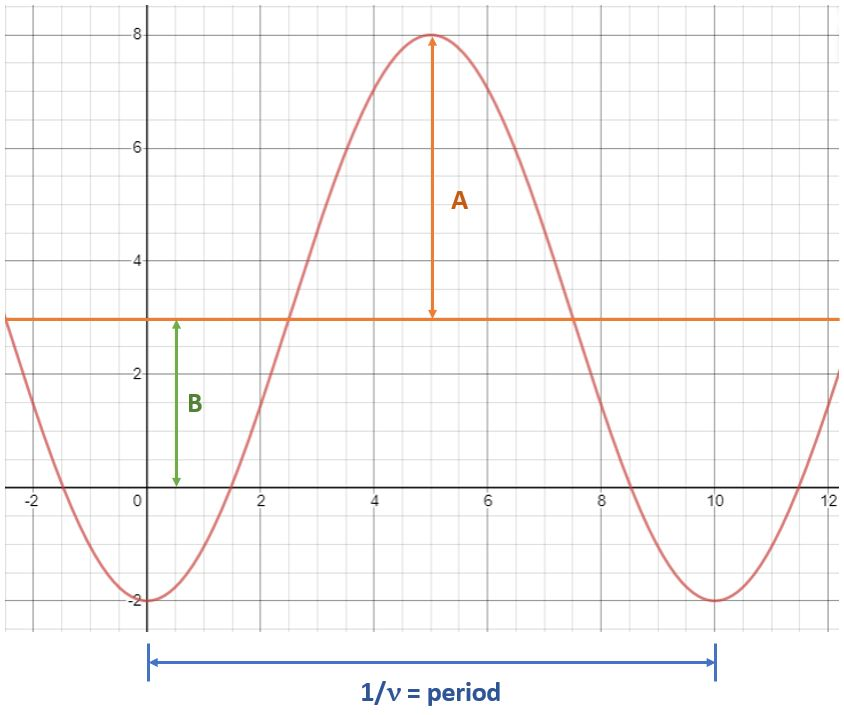
\includegraphics[scale=0.25]{fig/sin.jpg}
\end{center}

\begin{center}
$y = A * sin(2*\pi*\nu*t) + B$
\end{center}

where A = amplitude, B = offset, $\nu$ = frequency = $\frac{1}{period}$, 

and t = time in seconds.
\end{frame}


\begin{frame}\frametitle{Using Desmos (desmos.com/calculator)}
\begin{center}
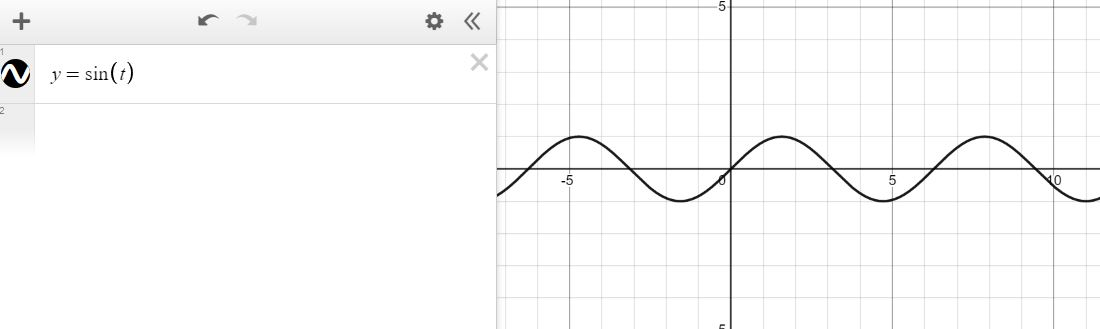
\includegraphics[scale=0.35]{fig/desmos1.jpg}
\end{center}
\begin{center}

\vspace{0.5cm}

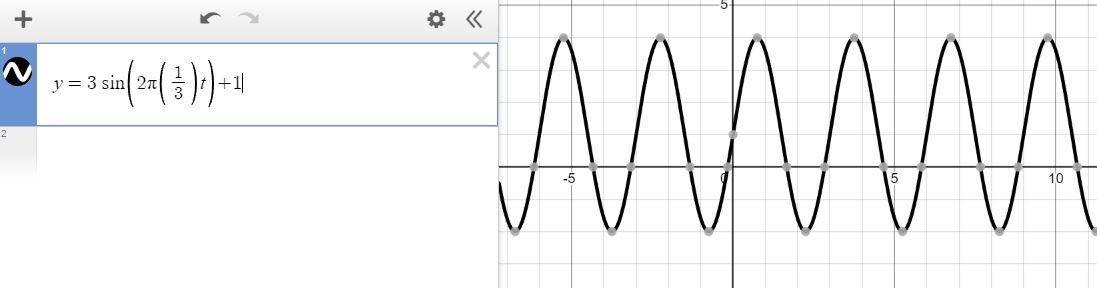
\includegraphics[scale=0.35]{fig/desmos2.jpg}
\end{center}
\end{frame}

\begin{frame}\frametitle{Phase Shift}
The sine wave can be shifted relative to each other by adding in a phase shift ($\phi$), which will shift the wave to the left or right.

Blue lags Red: 
\begin{center}
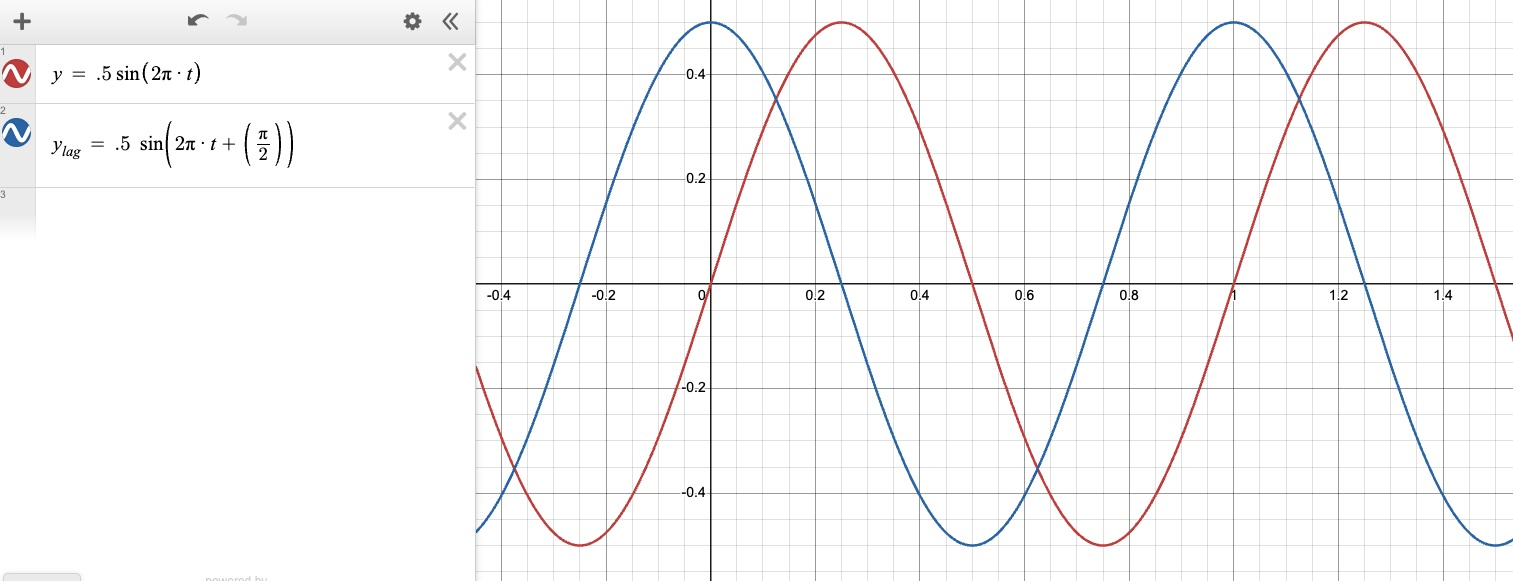
\includegraphics[height=2.6cm]{fig/sin_lag.jpg}
\end{center}

Green leads Red: 
\begin{center}
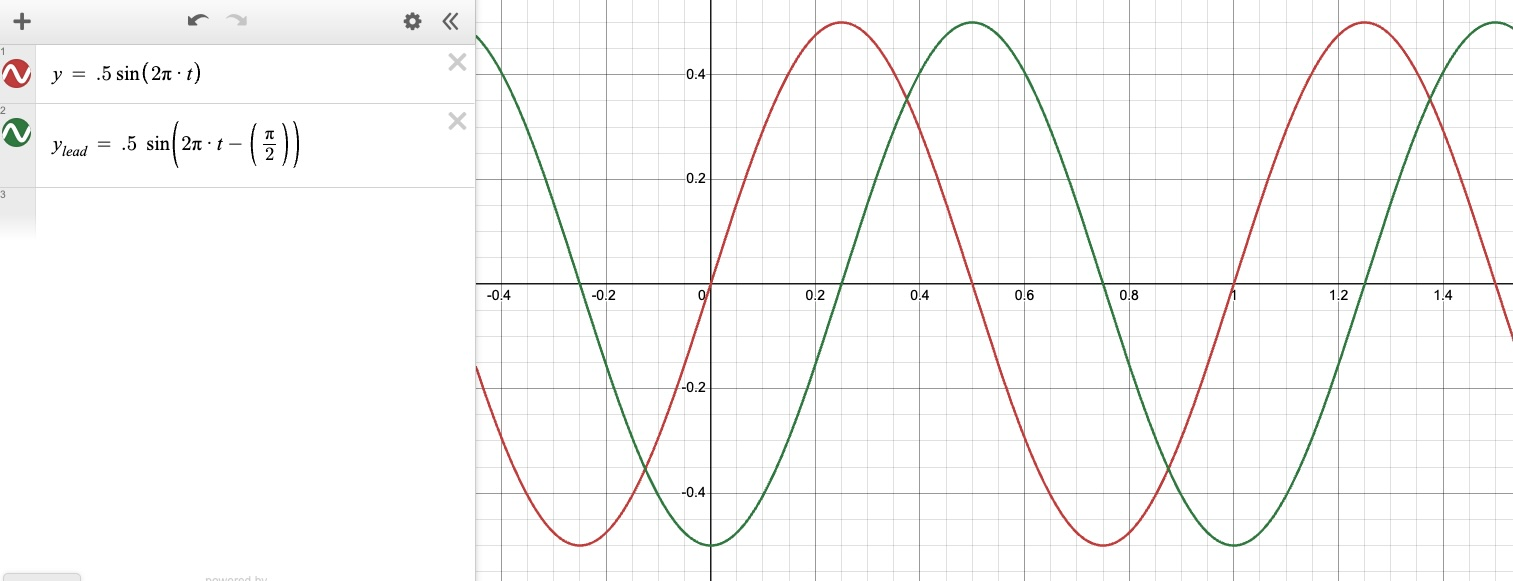
\includegraphics[height=2.6cm]{fig/sin_lead.jpg}
\end{center}

\end{frame}




\begin{frame}\frametitle{SOH CAH TOA}

\begin{itemize}
\item sin = opposite over hypotenuse
\item cos = adjacent over hypotenuse
\item tan = opposite over adjacent
\end{itemize}

\vspace{0.25cm}

\begin{center}
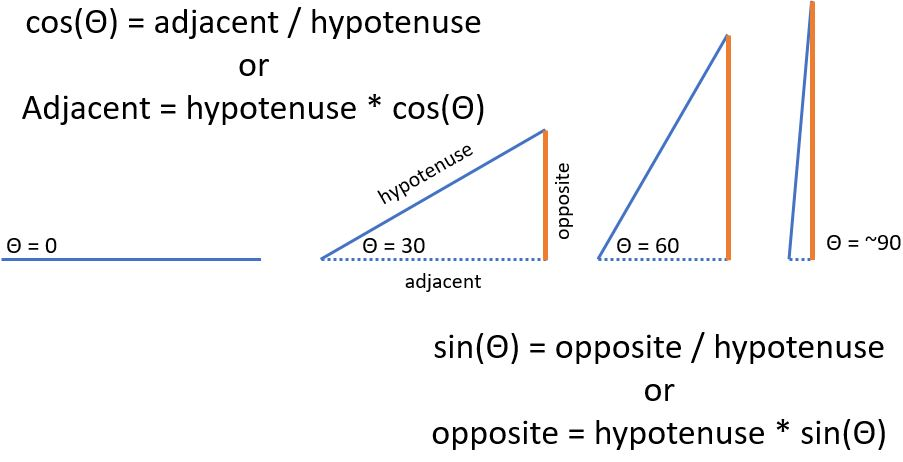
\includegraphics[scale=0.35]{fig/sohcahtoa.jpg}
\end{center}
\end{frame}

\begin{frame}\frametitle{Assignment: Calculating Angles: Laser Billards}
\begin{columns}
\begin{column}{4cm}
\begin{center}
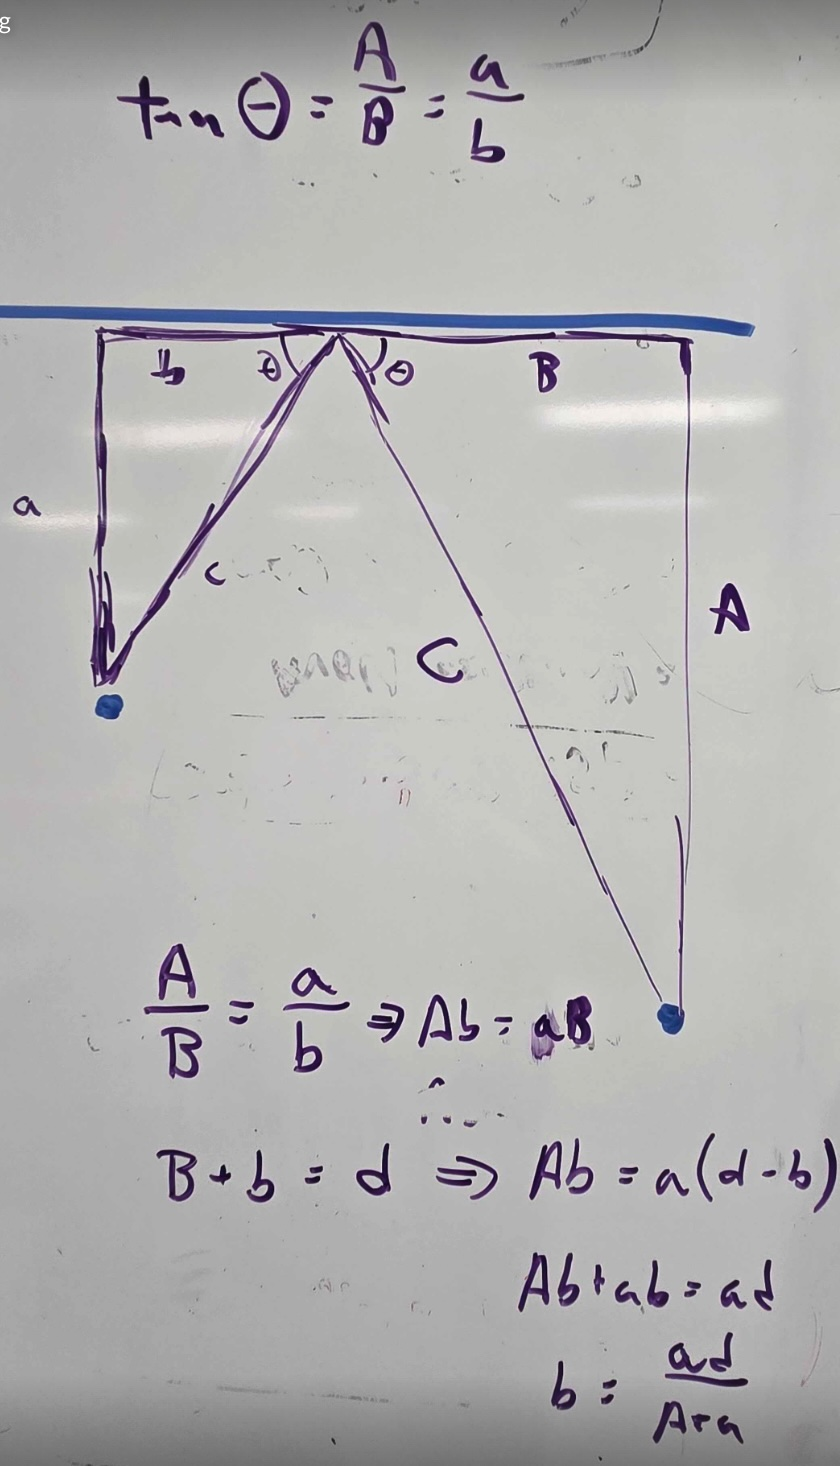
\includegraphics[width=4cm]{fig/billards.jpg}
\end{center}
\end{column}
\begin{column}{7cm}
\begin{itemize}
\item Setup a mirror line on the optical table.
\item Place the laser and target two different distances from the line.
\item Calculate the location of the mirror, place the mirror there.
\item Calculate the angle of the laser, adjust laser angle.
\item Turn on laser and see how close on target the calculations are.
\end{itemize}
\end{column}
\end{columns}
\end{frame}


\section{Return to Geometric Optics}

\begin{frame}\frametitle{Refraction}
The changing of a light ray’s direction (loosely called bending) when it passes through variations in matter is called refraction.

\begin{center}
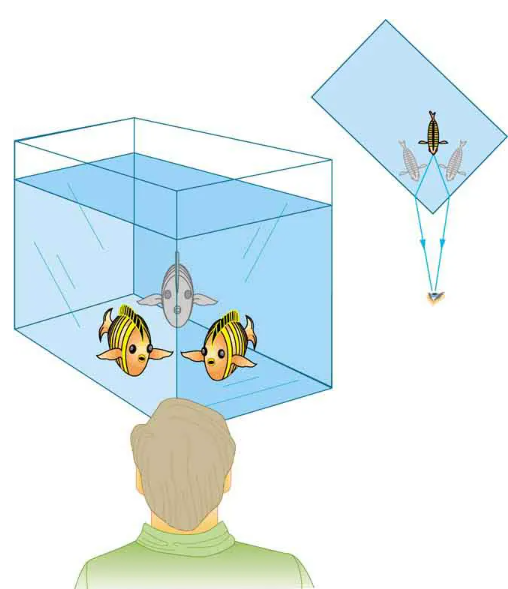
\includegraphics[width=5cm]{fig/fish.png}
\end{center}

\end{frame}


\begin{frame}\frametitle{Index of Refraction}

\begin{columns}
\begin{column}{6.5cm}
The speed of flight depends strongly on the type of material. We define the index of refraction ($n$) as

\begin{center}
$n = \frac{c}{v}$
\end{center}

where $v$ is the speed of light in the material and $c$ is the speed of light in a vacuum.
\end{column}
\begin{column}{5cm}
\begin{center}
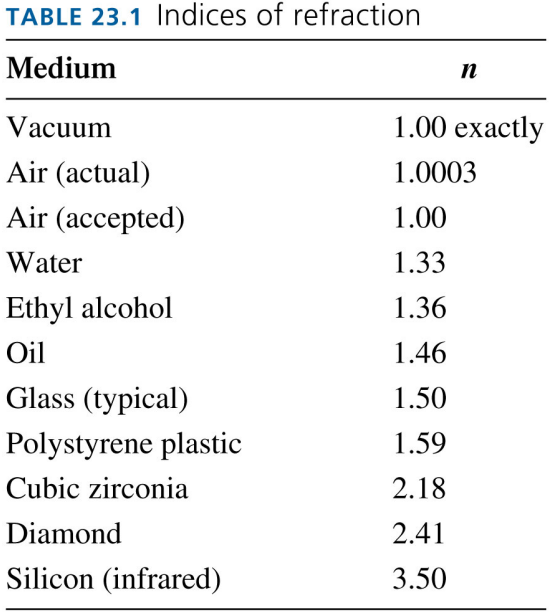
\includegraphics[width=5cm]{fig/n_table.png}
\end{center}
\end{column}
\end{columns}
\end{frame}

\begin{frame}\frametitle{Law of Refraction - Snell's Law}
The law of refraction is also called Snell’s law after the Dutch mathematician Willebrord Snell (1591–1626).

\begin{center}
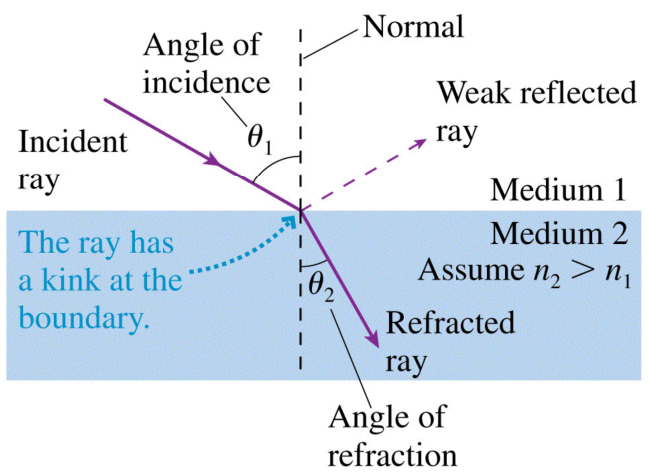
\includegraphics[width=6cm]{fig/snell.png}
\end{center}

\begin{center}
Snell's Law: $n_1 \sin{\theta_1} = n_2 \sin{\theta_2}$
\end{center}


\end{frame}

\begin{frame}\frametitle{Finding Index of Refraction}

Snells Law:

\begin{equation}
n_1 \sin{\theta_1} = n_2 \sin{\theta_2}
\end{equation}

Rearranging to isolate $n_2$:

\begin{equation}
n_2 = n_1 \frac{\sin{\theta_1}}{\sin{\theta_2}}
\end{equation}

For example, if the initial medium is air, $\theta_1 = 30^\circ \textdegree$ and $\theta_2 = 22^\circ$

\begin{equation}
n_2 = (1.00) \cdot \frac{\sin{30^\circ}}{\sin{22^\circ}} = \frac{0.500}{0.375} = 1.33
\end{equation}

\end{frame}

\begin{frame}\frametitle{Assignment: Measuring Refraction}
\begin{columns}
\begin{column}{4cm}
\begin{center}
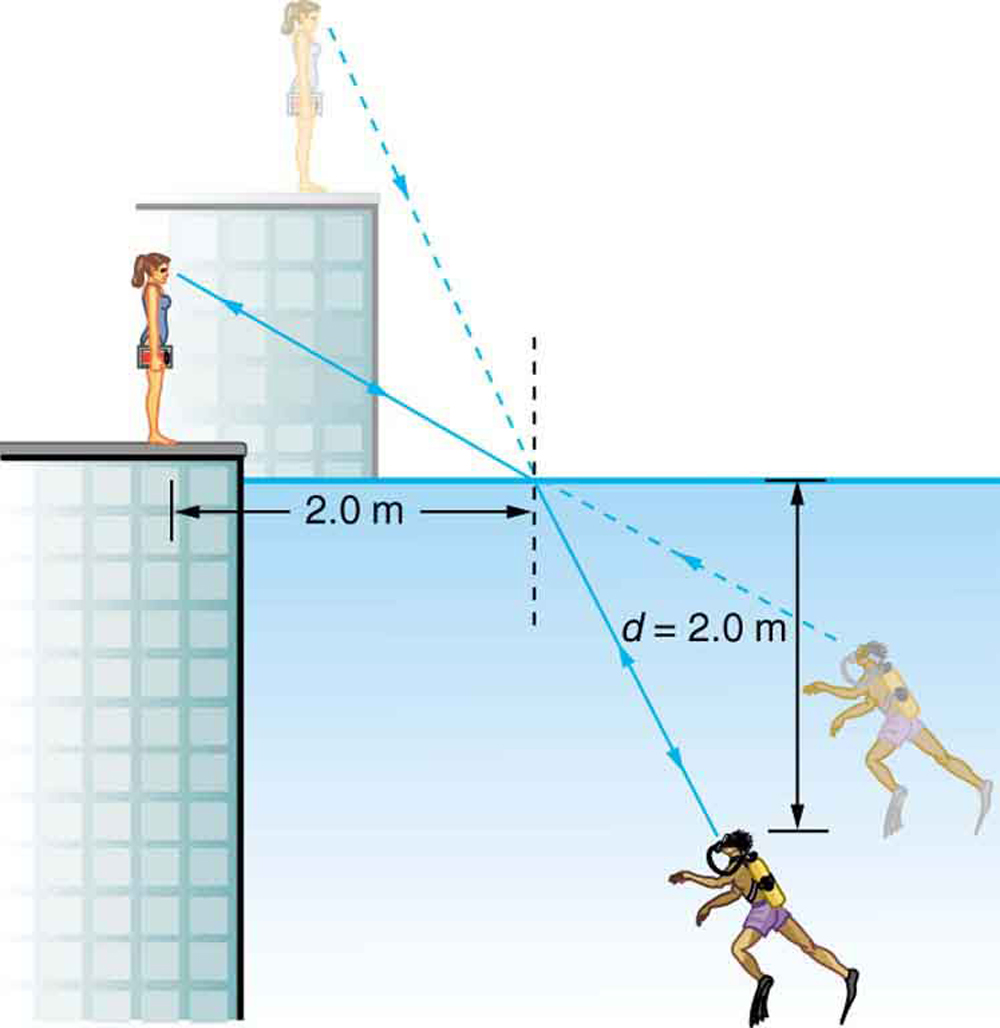
\includegraphics[width=4cm]{fig/refract9.jpg}
\end{center}
\end{column}
\begin{column}{7cm}
\begin{itemize}
\item Some assignment on refraction
\item Acrylic, water, what else?
\item Different color lasers (red, green, and if we get blue in time)
\end{itemize}
\end{column}
\end{columns}
\end{frame}


\begin{frame}\frametitle{Total Internal Reflection}

\begin{columns}
\begin{column}{9.5cm}
Good mirrors reflect $>90$\% of the light; however, total reflection can be produced via refraction.\newline

If the index of refraction of the second medium is less than that of the first medium, the rays are refracted away from the perpendicular. 

\begin{itemize}
\item Since $n_1 > n_2$, the angle of refraction is greater than the angel of incidence: $\theta_2 > \theta_1$.
\item Increasing $\theta_1$ causes $\theta_2$ to increase.
\item The critical angle ($\theta_c$) is defined to be the incident angle ($\theta_1$) that produces a $\theta_2 = 90^\circ$ 
\end{itemize}

The critical angle is given by:
\begin{equation}
\theta_c = sin^{-1}(\frac{n_2}{n_1}), \hspace{3mm} \text{for} \hspace{2mm}  n_1 > n_2
\end{equation}

\end{column}
\begin{column}{3cm}
\begin{center}

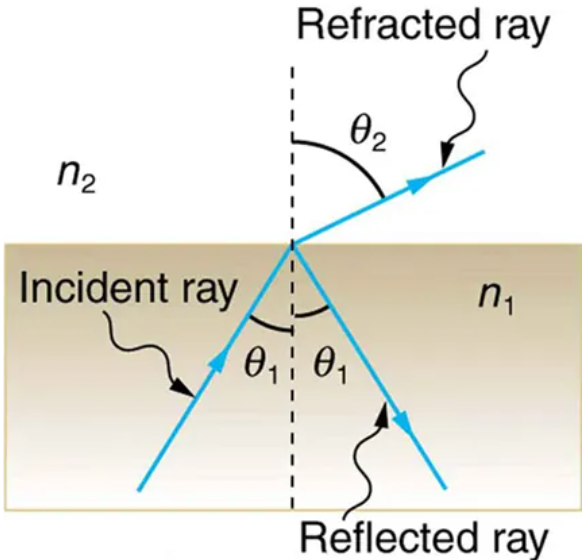
\includegraphics[width=2.5cm]{fig/tir1.png}

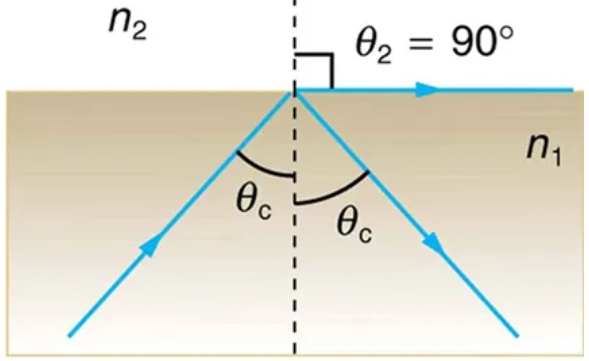
\includegraphics[width=2.5cm]{fig/tir2.png}

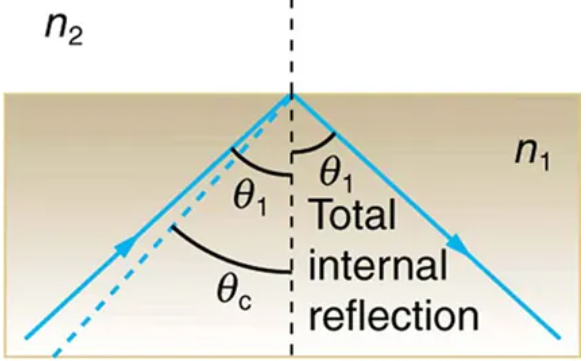
\includegraphics[width=2.5cm]{fig/tir3.png}

\end{center}
\end{column}
\end{columns}
\end{frame}


\begin{frame}\frametitle{Fiber Optic Cable}
The fiber optic cable takes advantage of the core having a high index of refraction than the cladding.

\begin{center}
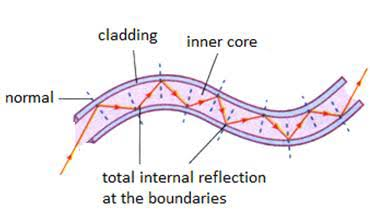
\includegraphics[width=6cm]{fig/cladding.jpg}
\end{center}

\vspace{3cm}

More to come on fibers as we progress through the Quantum Journey
\end{frame}

\begin{frame}\frametitle{Fiber: Acceptance Angle}
For multi-mode fibers, the numerical appeture (NA) provides  a good estimate of the maximum acceptance angle. 
\begin{columns}
\begin{column}{7cm}


\begin{itemize}
\item The cutoff angle is the maximum acceptance angle ($\theta_{max}$), which is related to NA:
\[ NA = n_0 sin(\theta_{max}) = \sqrt{n_{core}^2 + n_{clad}^2} \]

\item Rays with an angle of incidence $\leq \theta_{max}$ are totally internally reflected (TIR) at the fiber core/cladding boundary.

\item Rays with an angle of incidence $> \theta_{max}$ refract at and pass through the boundary.

\end{itemize}

\end{column}
\begin{column}{4cm}
\begin{center}

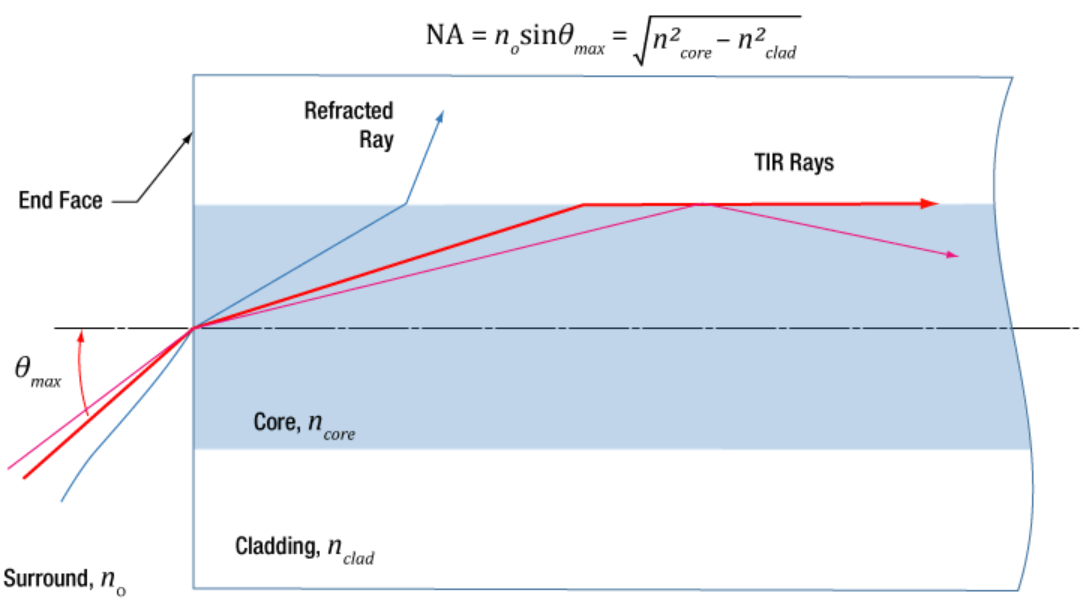
\includegraphics[width=3.8cm]{fig/fiber_NA.png}

\vspace{0.25cm}

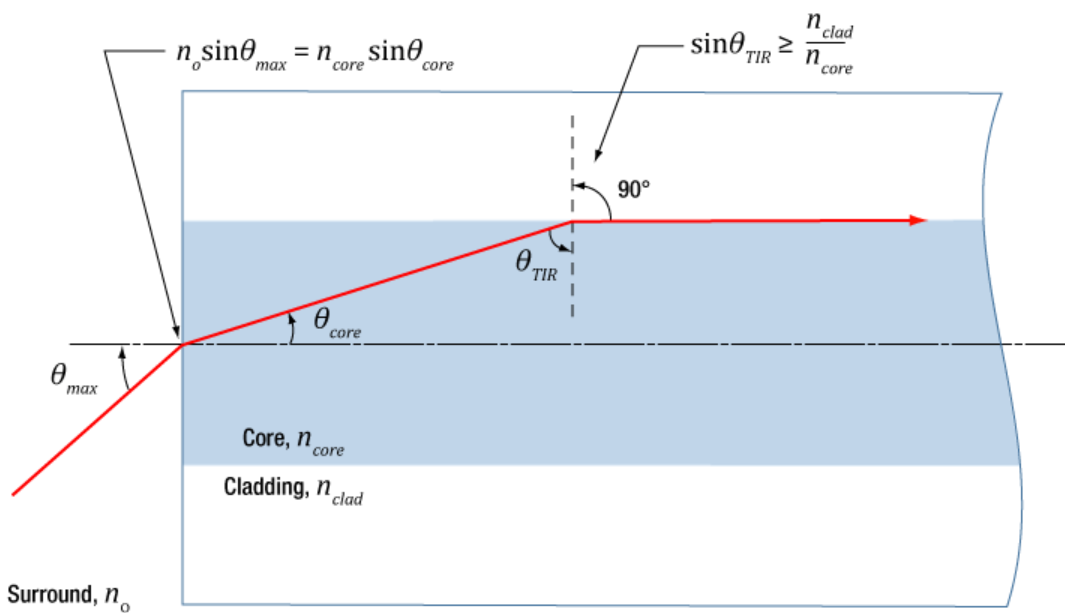
\includegraphics[width=3.8cm]{fig/fiber_TIR.png}

\end{center}
\end{column}
\end{columns}
\end{frame}


\begin{frame}\frametitle{Assignment: Fiber Coupling}
\begin{columns}
\begin{column}{4.5cm}
\begin{center}
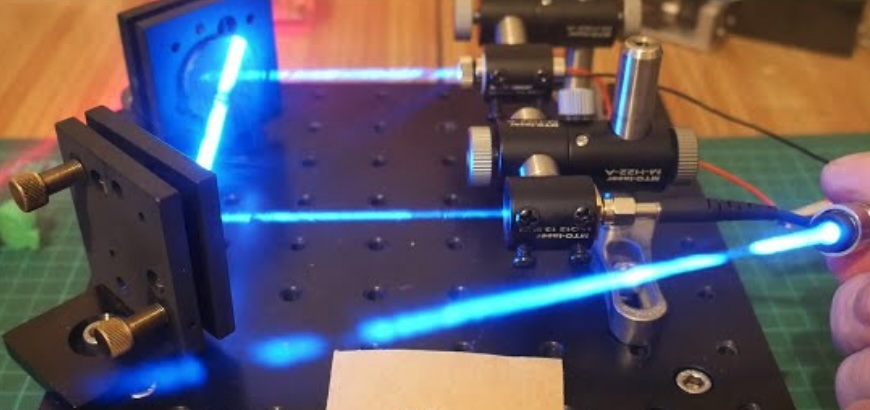
\includegraphics[width=4.5cm]{fig/coupling.jpg}

\vspace{1cm}

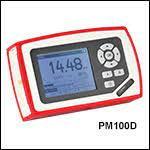
\includegraphics[width=3cm]{fig/pm100d.jpg}

\end{center}
\end{column}
\begin{column}{6.5cm}
\begin{itemize}
\item Use the two mirror walk to align a HeNe laser beam to a fiber.
\item Improve the quality of the coupling by maximizin the power meter reading.
\item How can you improve the coupling? 
\end{itemize}


\end{column}
\end{columns}

\end{frame}



\begin{frame}\frametitle{Dispersion}
Dispersion is defined to be the spreading of white light into its full spectrum of wavelengths.

\begin{center}
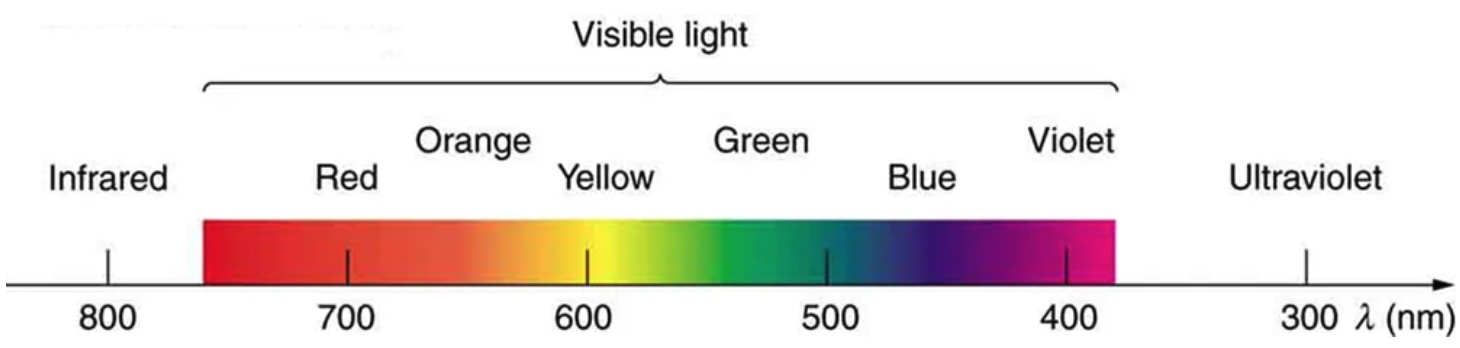
\includegraphics[width=10cm]{fig/rainbow.jpg}
\end{center}

\begin{itemize}
\item The angle of refraction depends on the index of refraction.
\item The index of refraction (n) depends on the properties of the medium.
\item However, for a given medium, n also depends on the optical wavelength.
\end{itemize}


\end{frame}

\begin{frame}\frametitle{Index of Refraction by Wavelength}
Index of refraction ($n$) by wavelength ($\lambda$):

\begin{center}
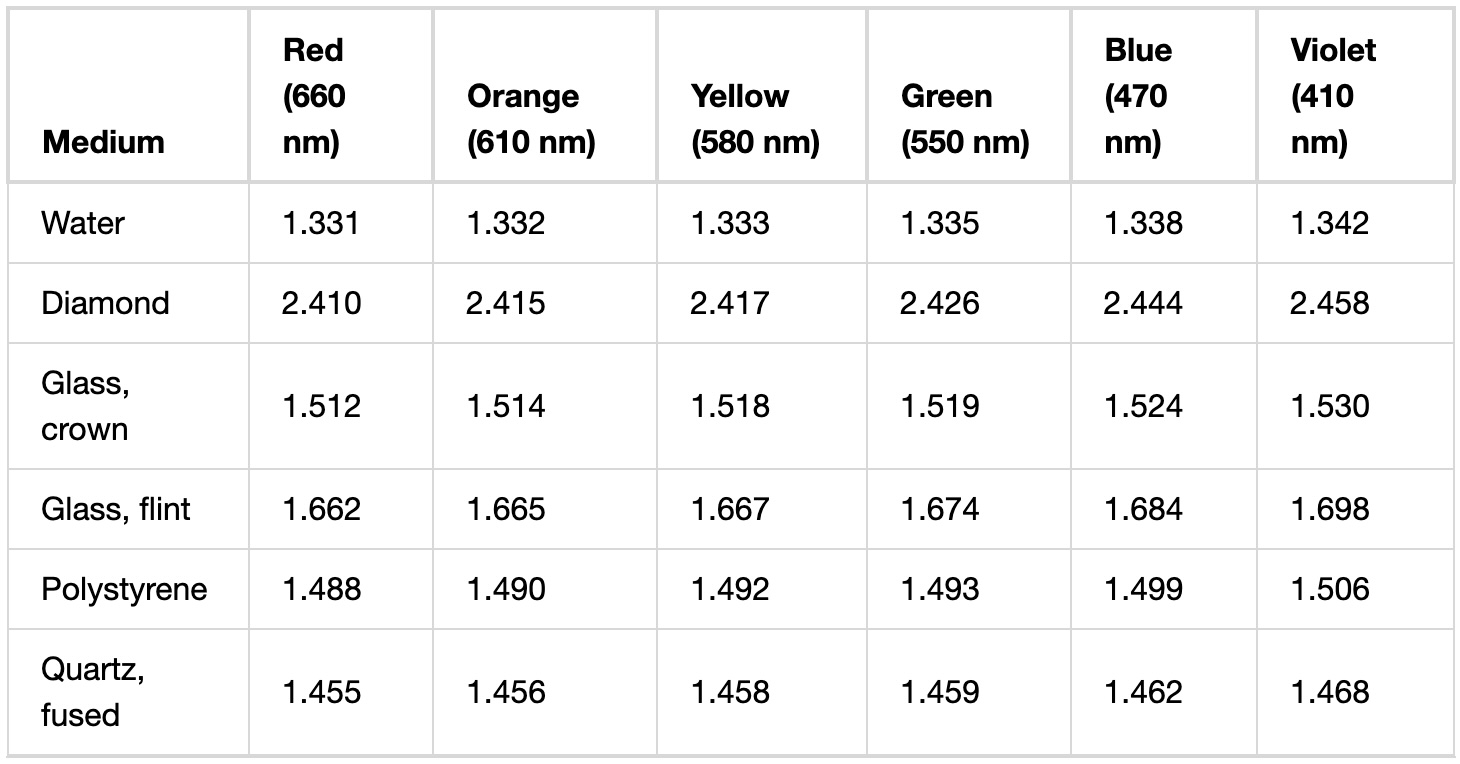
\includegraphics[width=10cm]{fig/nbylambda.jpg}
\end{center}
\end{frame}


\begin{frame}\frametitle{Glass Prism}
\begin{columns}
\begin{column}{5.5cm}
\begin{center}
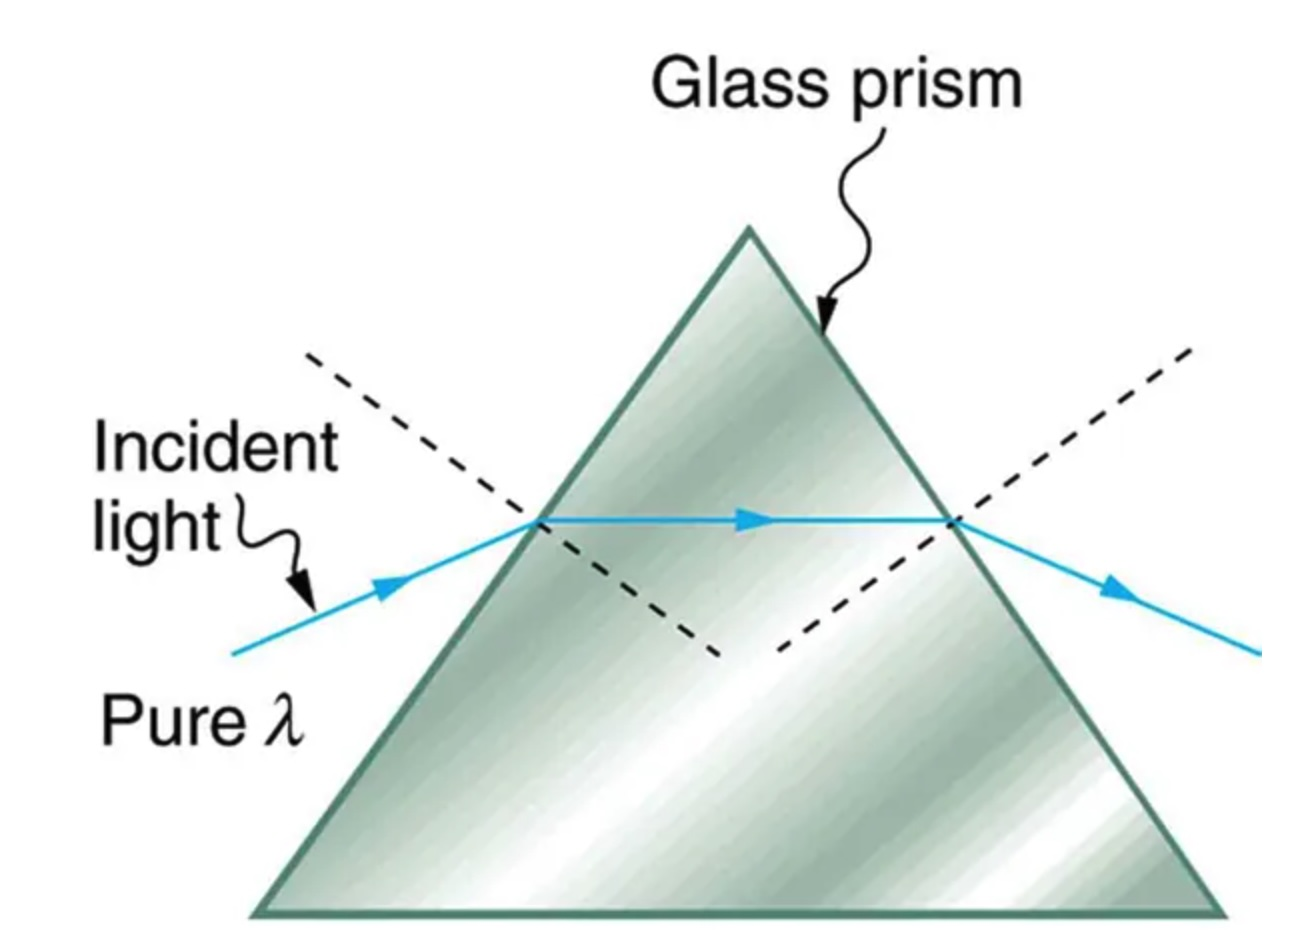
\includegraphics[height=3.6cm]{fig/gpideal.jpg}
\end{center}
\end{column}
\begin{column}{5.5cm}
\begin{center}
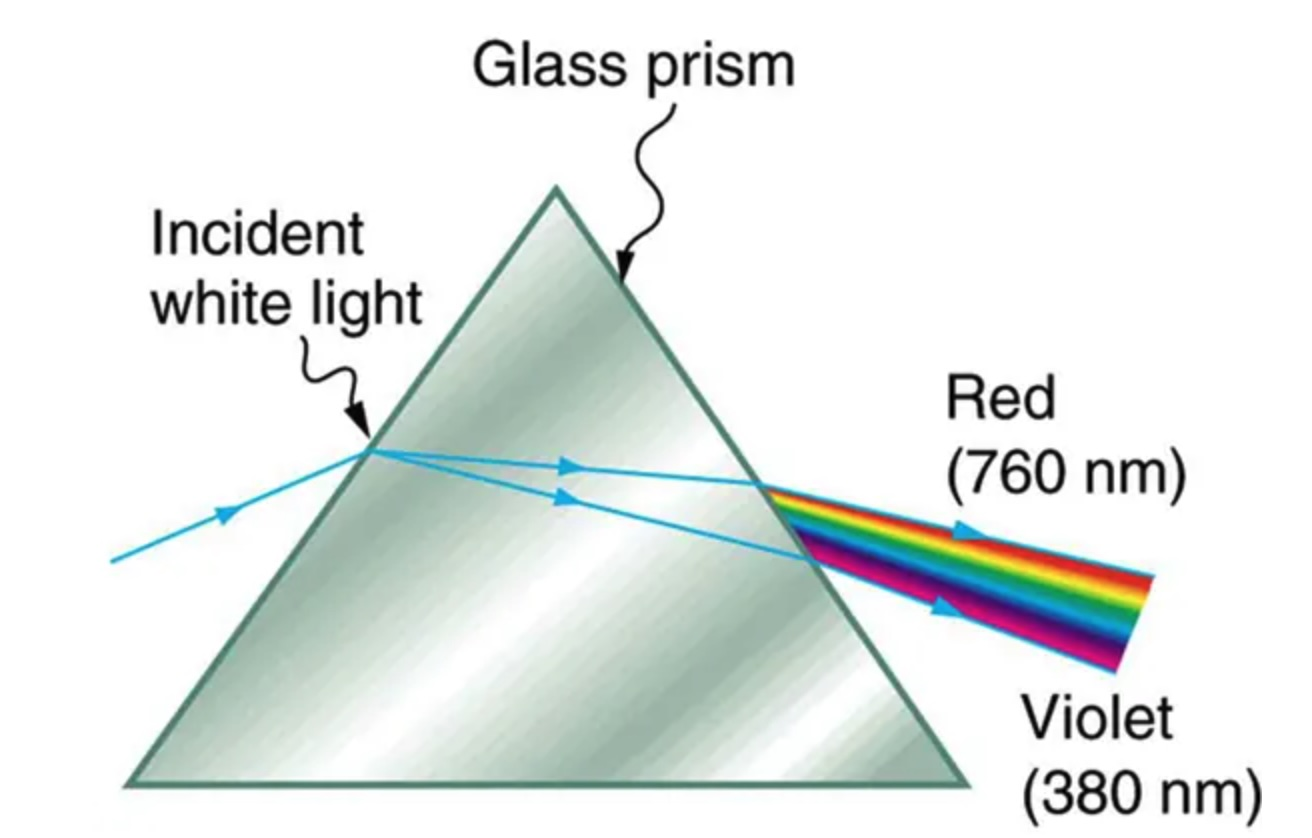
\includegraphics[height=3.7cm]{fig/gpreal.jpg}
\end{center}
\end{column}
\end{columns}
\end{frame}

\begin{frame}\frametitle{Rainbow}
\begin{center}
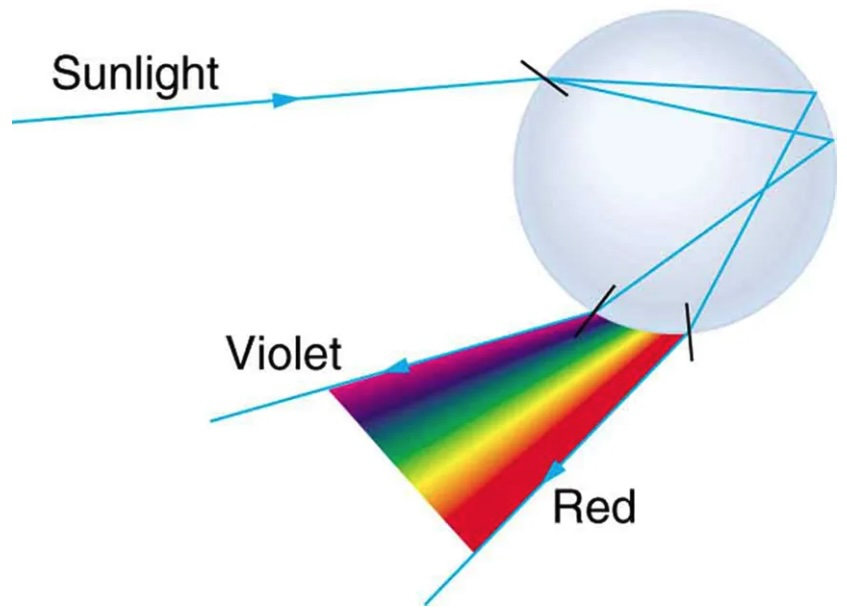
\includegraphics[width=6cm]{fig/rainbow2.jpg}
\end{center}
Rainbows are produced by a combination of refraction and reflection. You may have noticed that you see a rainbow only when you look away from the sun. Light enters a drop of water and is reflected from the back of the drop. The light is refracted both as it enters and as it leaves the drop. Since the index of refraction of water varies with wavelength, the light is dispersed, and a rainbow is observed.
\end{frame}

\begin{frame}\frametitle{Rainbow as an Arc}
\begin{columns}
\begin{column}{5.5cm}
\begin{center}
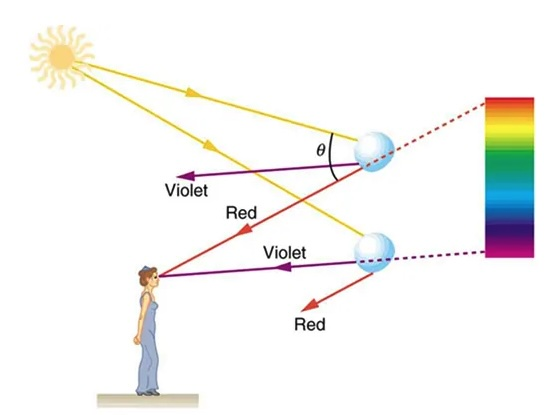
\includegraphics[width=5cm]{fig/rainbow3.jpg}
\end{center}
\end{column}
\begin{column}{5.5cm}
\begin{center}
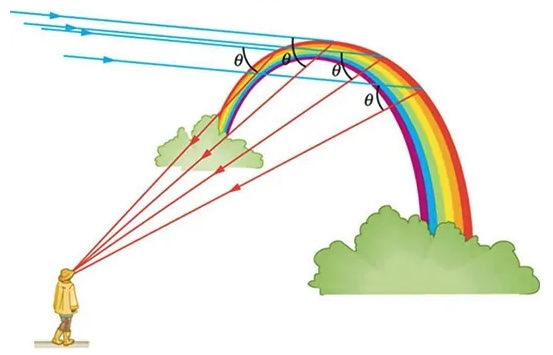
\includegraphics[width=5cm]{fig/rainbow4.jpg}
\end{center}
\end{column}
\end{columns}
\end{frame}


\section{Lens}

\begin{frame}\frametitle{Lens}
With the Law of Refraction, we can explore the properties of lens and how images are formed.
\begin{columns}
\begin{column}{6.5cm}
\begin{itemize}
\item The word lens comes from the Latin word for lentil bean, the shape of which is similar to a convex lens.
\item Convex Lens: all light rays that enter parallel to the axis cross one another at  a single point on the opposite side of the lens, i.e., they converge.
\item Concave Lens: all light rays that enter parallel to the axis diverge (bend away) from the lens axis.
\end{itemize}
\end{column}
\begin{column}{4.5cm}
\begin{center}
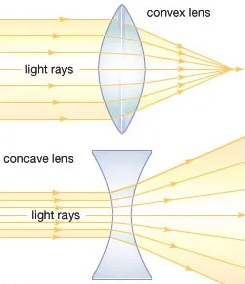
\includegraphics[width=4cm]{fig/cavevex.jpg}
\end{center}
\end{column}
\end{columns}
\end{frame}


\begin{frame}\frametitle{Convex Lens}
With the Law of Refraction, we can explore the properties of lens and how images are formed.
\begin{columns}
\begin{column}{6cm}
\begin{itemize}
\item A ray of light bends (refracts) at both interface, and for convex lens converge.
\item The point at which the rays crossed is defined as the Focal point ($F$) of the lens.
\item The distance from the center of the lens to its focal point is called the focal length ($f$).
\item The Power of the lens, measuring in Diopters ($P=\frac{1}{f}$) where $f$ is measured in meters.
\end{itemize}
\end{column}
\begin{column}{5cm}
\begin{center}
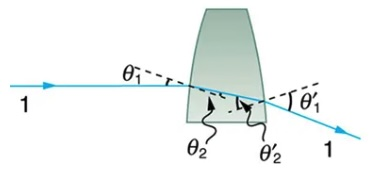
\includegraphics[width=4cm]{fig/convex1.jpg}

\vspace{0.25cm}
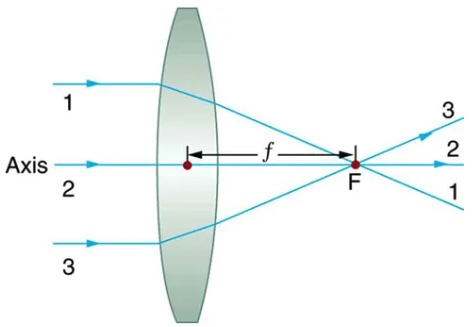
\includegraphics[width=4cm]{fig/convex2.jpg}
\end{center}
\end{column}
\end{columns}
\end{frame}

\begin{frame}\frametitle{Concave Lens}
\begin{columns}
\begin{column}{6cm}
\begin{itemize}
\item A concave lens is a diverging lens, it causes light rays to bend away from the axis.
\item In the case of all rays entering parallel to its axis, the light appears to originate at the same point $F$.
\item The distance from the center of the lens to its focal point is called the focal length ($f$) and is defined to be negative.
\end{itemize}
\end{column}
\begin{column}{5cm}
\begin{center}
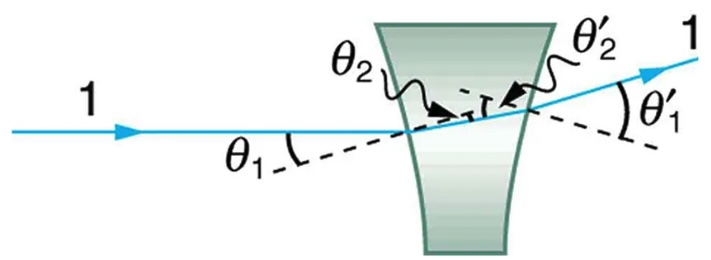
\includegraphics[width=4cm]{fig/concave1.jpg}

\vspace{0.25cm}
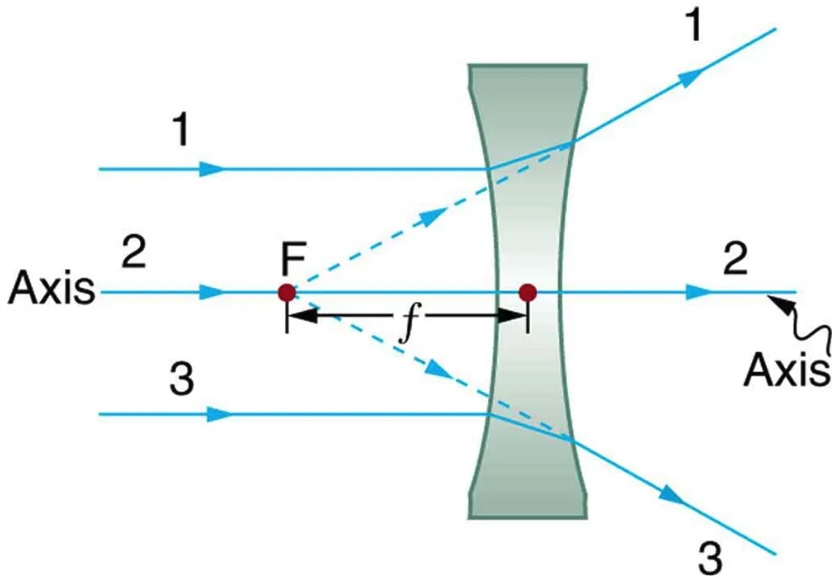
\includegraphics[width=4cm]{fig/concave2.jpg}
\end{center}
\end{column}
\end{columns}
\end{frame}


\begin{frame}\frametitle{Assigment: Find the Focal Length}
\begin{columns}
\begin{column}{4.6cm}
\begin{center}
\includegraphics[width=4.5cm]{fig/sunfire.jpg}
\end{center}
\end{column}
\begin{column}{7.4cm}
\begin{itemize}
\item Using some random lens, use the overhead lighting to find the focal length
\item Repeat on optical table using laser
\item Clean lens before putting away
\end{itemize}
\end{column}
\end{columns}
\end{frame}

\begin{frame}\frametitle{Thin Lens}
A thin lens is defined to be one whose thickness allows rays to refract but does not allow properties such as dispersion and aberrations.
\end{frame}

\begin{frame}\frametitle{Ray Tracing}
\begin{columns}
\begin{column}{7.4cm}
\begin{enumerate}
\item A ray entering a converging lens parallel to its axis passes through the focal point F of the lens on the other side.
\item A ray entering a diverging lens parallel to its axis seems to come from the focal point F.
\item A ray passing through the center of either a converging or a diverging lens does not change direction.
\item A ray entering a converging lens through its focal point exits parallel to its axis.
\item A ray that enters a diverging lens by heading toward the focal point on the opposite side exits parallel to the axis.
\end{enumerate}


\end{column}
\begin{column}{4.6cm}
\begin{center}
\includegraphics[width=4.5cm]{fig/raytrace.jpg}
\end{center}
\end{column}
\end{columns}
\end{frame}


\begin{frame}\frametitle{Image Formation}

\begin{center}
\includegraphics[width=8cm]{fig/imageform1.jpg}
\end{center}


Thin Lens equations:

\begin{columns}
\begin{column}{5.5cm}
\[ \frac{1}{d_o} + \frac{1}{d_i} = \frac{1}{f}\]
\end{column}
\begin{column}{5.5cm}
\[ \frac{h_i}{h_o} = -\frac{d_i}{d_o} = m\]
\end{column}
\end{columns}

\end{frame}


\begin{frame}\frametitle{Image Formation - Real Image}
\begin{columns}
\begin{column}{5.5cm}
\begin{center}
\includegraphics[width=5cm]{fig/imageform2.jpg}
\end{center}
\end{column}
\begin{column}{5.5cm}
\begin{center}
\includegraphics[width=5cm]{fig/imageform3.jpg}
\end{center}
\end{column}
\end{columns}

\vspace{1cm}

The image in which light rays from one point on the object actually cross at the location of the image and can be projected onto a screen, a piece of film, or the retina of an eye is called a real image.

\end{frame}

\begin{frame}\frametitle{Assignment - Focus CCD Camera}
\begin{columns}
\begin{column}{4.5cm}
\begin{center}
\includegraphics[width=4cm]{fig/thorCCD.jpg}
\end{center}
\end{column}
\begin{column}{7cm}
\begin{itemize}
\item
\item 
\end{itemize}
\end{column}
\end{columns}
\end{frame}


\begin{frame}\frametitle{Image Formation - Virtual Image}

\begin{center}
\includegraphics[width=8cm]{fig/imageform4.jpg}
\end{center}

If an object is held closer to the converging lens than its focal length ($f$), then the rays from a common point continue to diverge after passing through the lens. They all appear to originate from a point at the location of the image, on the same side of the lens as the object. This is a virtual image. 


\end{frame}

\begin{frame}\frametitle{Image Formation - Concave Lens}

\begin{center}
\includegraphics[width=8cm]{fig/imageform5.jpg}
\end{center}
\end{frame}


\begin{frame}\frametitle{Beam Expander/Reducer - Telescope}
\begin{columns}
\begin{column}{5.5cm}
\begin{center}
\includegraphics[width=5cm]{fig/beamXkepler.png}
Galilean Design
\end{center}
\end{column}
\begin{column}{5.5cm}
\begin{center}
\includegraphics[width=5cm]{fig/beamXgalileo.png}
Galilean Design
\end{center}
\end{column}
\end{columns}

\vspace{0.25cm}
Both the bean's waist ($2W_0$) and the divergence angle ($\theta$) are affected by by the beam expanders and reducers. If Lens 2 is the output lens, then the beam expansion ratio ($m_{12}$) is: 
\begin{equation}
m_{12} = \frac{f_2}{f_1}
\end{equation}

\end{frame}



\section{Math Interlude: Probability}

\begin{frame}\frametitle{Probability and Statistics}
\begin{columns}
\begin{column}{5cm}
\begin{center}
\includegraphics[width=5cm]{fig/cartoonguidestats.jpg}
\end{center}
\end{column}
\begin{column}{5cm}
\begin{itemize}
\item Data Analysis: The gathering, display, and summary of data
\item Probability: The laws of chance (inside and outside of a casino)
\item Statistical Inference: the science of drawing statistical conclusions from specific data using the laws of probability
\end{itemize}
\end{column}
\end{columns}
\end{frame}

\begin{frame}\frametitle{A Tale as Old as Time}
\begin{center}
\includegraphics[width=6cm]{fig/vegas.jpg}
\end{center}


Gambling is as old as mankind, so it seems that probability should be almost as old. But, the realization that one could predict an outcome to a certain degree of accuracy was unconceivable until the $16^{th}$ century. In order to make a profit, underwriters were in need of dependable guidelines by which a profit could be expected, while the gambler was interested in predicting the possibility of gain.
\end{frame}



\begin{frame}\frametitle{Rich Guys Gambling}
\begin{columns}
\begin{column}{4cm}
\begin{center}
\includegraphics[width=3cm]{fig/cardano.jpg}
\end{center}
\end{column}
\begin{column}{7.5cm}
Known as the “Father of Probability”, Gerolamo Cardano was an Italian mathematician, physician, and gambler who first talked about probability. Cardano’s fascination with games of chance led him to write the first book dedicated to probability, “Liber de Ludo Aleae” (Book on Games of Chance), published in 1564. Cardano introduced concepts like odds and probabilities in this work, providing a framework for analyzing the likelihood of different outcomes in dice rolls and other games.
\end{column}
\end{columns}
\end{frame}

\begin{frame}\frametitle{Probability}


\begin{columns}
\begin{column}{5cm}
The probability of an event expresses the likelihood of the event outcome

\[P(event) = \frac{\text{\# of favorable outcomes}}{\text{\# of all possibly outcomes}}\]
\end{column}
\begin{column}{5cm}
\begin{center}
\includegraphics[width=3cm]{fig/coinflip.jpg}
\end{center}
\end{column}
\end{columns}
\end{frame}

\begin{frame}\frametitle{Frequency Tables and Histograms}

\begin{center}

Roll two dice and add them together, repeat. \newline

\includegraphics[width=10cm]{fig/stat1.jpg}
\end{center}

\end{frame}

\begin{frame}\frametitle{Assignment: Tenzi}
\begin{columns}
\begin{column}{4cm}
\begin{center}
\includegraphics[width=4cm]{fig/dice.jpg}
\end{center}
\end{column}
\begin{column}{7cm}

Role two dice 12 times, after each role:
\begin{itemize}
\item Record the sum
\item Record the running average (total up to this point divided by number of roles)
\end{itemize}
After the twelfth role:
\begin{itemize}
\item Create a histogram of the sums
\item Create a line chart of the running averages
\end{itemize}
\end{column}
\end{columns}
\end{frame}


\begin{frame}\frametitle{Summary Statistics}


\begin{columns}
\begin{column}{7cm}
\begin{itemize}
\item Mean (or average): add the totals and divide by number of samples
\[ \bar{x} = \frac{x_1 + x_2 + x_3 + ... + x_n}{n} \]
or
\[ \bar{x} = \frac{\sum_{i=1}^{n} (x_i)}{n}\]
\item Median: middle sample in the ordered distribution
\begin{itemize}
\item Odd: median is the value of middle sample
\item Even: median is the average of the two middle samples
\end{itemize}
\item Mode: the value the appears most often
\end{itemize}
\end{column}
\begin{column}{4cm}
\begin{center}
\includegraphics[width=4cm]{fig/stat2.jpg}


average = $\bar{x} = 7$

median $= 6$

mode $ = 6$
\end{center}
\end{column}
\end{columns}
\end{frame}


\begin{frame}\frametitle{Summary Statistics: Variation}
\begin{center}
\includegraphics[width=11cm]{fig/stat3.jpg}
\end{center}
\begin{itemize}
\item Interquartile Range (IRQ): Spread of the middle $50\%$ of the data
\begin{itemize}
\item Find the median
\item Find the first quartile (Q1): median of the lower half.
\item Find the third quartile (Q3): median of the upper half.
\item IRQ = Q3 - Q1 = 6
\end{itemize}


\item Standard Deviations ($\sigma$):
\[ \sigma = \sqrt{ \frac{ \sum_{i=0}^n (x_i - \bar{x})^2}{n}} = 3.06\]

\end{itemize}

\end{frame}


\begin{frame}\frametitle{Gaussian Distribution}

\begin{center}
\includegraphics[width=6cm]{fig/stat4.png}
\end{center}

Probability Distribution Function $f(x)$:

\[ f(x) = \frac{1}{\sqrt{2 \pi \sigma^2}} e^{\frac{-(x-\bar{x})^2}{2 \sigma^2}} \]

\end{frame}

\begin{frame}\frametitle{Gaussian Distribution: $3 \sigma$}
\begin{columns}
\begin{column}{6cm}
\begin{center}
\includegraphics[width=6cm]{fig/stat5.png}
\end{center}
\end{column}
\begin{column}{4cm}

\begin{center}
Galton Baord
\includegraphics[width=4cm]{fig/stat7.png}
\end{center}
\end{column}
\end{columns}
\end{frame}

\begin{frame}\frametitle{Assignment: Measuring Bean Profile}
\begin{columns}
\begin{column}{4cm}
\begin{center}
\includegraphics[width=3cm]{fig/profile1.jpg}
\includegraphics[width=3cm]{fig/profile2.jpg}
\end{center}
\end{column}
\begin{column}{7cm}
The laser beam has a Gaussian profile.
\begin{enumerate}
\item Direct a laser beam at a power meter, setting the correct wavelength
\item Moving the knife edge across the beam path, record the drop in power vs distance.
\item Setup a telescope to expand the beam size by 2-5 times.
\item Repeat the knife edge process.
\item Plot the results of both sets of measurements on paper and in excel.
\end{enumerate}
\end{column}
\end{columns}
\end{frame}

\begin{frame}\frametitle{Python Excursion}

\begin{center}
\includegraphics[width=6cm]{fig/python1.png}
\end{center}

\end{frame}


\section{Mirrors}

\begin{frame}\frametitle{Flat Mirror}

\begin{center}
\includegraphics[width=10cm]{fig/mirrorimage1.jpg}
\end{center}

\end{frame}

\begin{frame}\frametitle{Concave Spherical Mirrors - Thin Lens Equivalent}

\begin{center}
\includegraphics[width=10cm]{fig/mirrorimage2.jpg}
\end{center}

For a mirror that is large compared to the radius of curvature, the reflected rays do not cross at the same point. A parabolic mirror, the rays would indeed cross at a single point. However, parabolic mirrors are expensive. So, using a mirror that is small compared to the radius of curvature, leads to a well-defined focal point $F$, with $f = \frac{R}{2}$.

\end{frame}

\begin{frame}\frametitle{Convex Mirrors}

\begin{center}
\includegraphics[width=5cm]{fig/mirrorimage3.jpg}
\end{center}

\end{frame}

\begin{frame}\frametitle{Image Formation - Concave Mirrors}

\begin{center}
\includegraphics[width=8cm]{fig/mirrorimage4.jpg}
\end{center}

\end{frame}

\begin{frame}\frametitle{Image Formation - Concave Mirrors}

\begin{center}
\includegraphics[width=8cm]{fig/mirrorimage5.jpg}
\end{center}

\end{frame}

\begin{frame}\frametitle{Image Formation - Convex Mirrors}

\begin{center}
\includegraphics[width=8cm]{fig/mirrorimage6.jpg}
\end{center}

\end{frame}

\section{Vision}

\begin{frame}\frametitle{The Eye}

\begin{center}
\includegraphics[width=6cm]{fig/theI.jpg}
\end{center}

\end{frame}

\begin{frame}\frametitle{Rods and Cones and Color}

\begin{center}
\includegraphics[width=6cm]{fig/rodscones.jpg}
\end{center}

\end{frame}

\begin{frame}\frametitle{Visible Spectrum}

\begin{center}
\includegraphics[width=10cm]{fig/visSpec.jpg}
\end{center}

\end{frame}

\begin{frame}\frametitle{Spectrum of Light Sources}

\begin{center}
\includegraphics[width=10cm]{fig/lightSpec.jpg}
\end{center}

\end{frame}

\begin{frame}\frametitle{Chromatic Aberrations}

\begin{center}
\includegraphics[width=10cm]{fig/chromeAbb.jpg}
\end{center}

\end{frame}

\begin{frame}\frametitle{Correcting Chromatic Aberrations}

\begin{center}
\includegraphics[width=10cm]{fig/chromeAbb2.jpg}
\end{center}

\end{frame}

\begin{frame}\frametitle{Coma - Off Axis Abberation}

\begin{center}
\includegraphics[width=10cm]{fig/coma.jpg}
\end{center}

\end{frame}

\begin{frame}\frametitle{Spherical Aberrations}

\begin{center}
\includegraphics[width=10cm]{fig/sphereAbb.jpg}
\end{center}

\end{frame}




\end{document}
